\chapter{Einrichtung und Betrieb}

GitHub Repositorium:

\begin{itemize}
  \item Dieses Dokument:\\
        \url{https://github.com/themerius/Bachelor-Thesis}
  \item DSL:\\
        \url{https://github.com/themerius/ScalTeX-DSL}
  \item Zielarchitetkur:\\
        \url{https://github.com/themerius/ScalTeX-templates}
\end{itemize}

Die einzelnen Versionsstände die von der Scala-DSL entstandenen sind,
sind auf meinem Google Drive gespeichert und können dort als ZIP
geladen werden:

\begin{enumerate}
  \item R1\\
        \url{http://goo.gl/hKjxu}
  \item R2\\
        \url{http://goo.gl/rQ7un}
  \item R3\\
        \url{http://goo.gl/k1bZm}
  \item R4\\
        \url{http://goo.gl/2QwWE}
  \item R5\\
        \url{http://goo.gl/CqFZP}
\end{enumerate}

\section{Voraussetzungen}

\begin{itemize}
  \item Java Virtual Machine bzw. OpenJDK in Version 6 oder 7,
  \item UNIX Betriebssystem,
  \item git,
  \item sbt.
\end{itemize}

\section{Ausführen}

\begin{enumerate}
  \item Mit git das Repositorium herunterladen (oder die o.g. ZIPs nehmen):\\
        \verb+git clone https://github.com/themerius/ScalTeX-DSL+
  \item In das \verb+ScalTeX-DSL/Scala-NextGen+ Verzeichnis wechseln,
  \item \verb+sbt+ ausführen,
  \item in der sbt-shell den Befehl \verb+run+ eingeben.
  \item (Mit \verb+test+ werden die Testszenarien ausgeführt.)
\end{enumerate}

Nach dem \verb+run+ Befehl werden von sbt automatisch die benötigten
Bibliothektsabhänigkeiten und korrekte Scala Version heruntergeladen.
Danach werden die Quellen kompiliert und ausgeführt---es sollte dann eine
\verb+_output/output.html+ Datei entstehen, mit dem Dokument als HTML-Datei,
welche die, hier im Dokument entstandene, Zielarchitektur verwendet.

In \verb+src/main/scala/main.scala+ liegt das
beispielhafte Dokumentenskript.

Im Repositorium der der Zielarchitektur sind die Tests für diese.
Dafür wird \verb+scaltex/TestSuite.html+ in einem Webbrowser
geöffnet. Der Webbrowser führt dann die JavaScript-Testsuite aus.


\chapter{Codebeispiele}

\section{Beispiel DSL-Skript}\label{sec-api-resultat}

\begin{lstlisting}[label=dsl-skript,caption=Ausführliches Scala DSL Dokument-Skript.]
import scaltex.template.fraunhofer._

object Doc extends FraunhoferReportBuilder {

  val toc = new TableOfContents(doc)
  val doc = new Document

  set document_name "Textsatzsysteme"
  set institut_name "Fraunhofer SCAI"

  KapitelTextsatz
  KapitelScaltex
  PythonPlot

  toc.create

  def main(args: Array[String]) {
    write("_output/output.html")
  }
}

object KapitelTextsatz extends Document {

  ++ § "Textsatzsysteme: Einleitung"

  ++ txt """
    Textsatzsysteme übernehmen „das rechnergestützte Setzen von Dokumenten,
    die aus Texten und Bildern bestehen und später als Publikationen,
    wie zum Beispiel Broschüren, Magazine, Bücher oder Kataloge,
    ihre Verwendung finden.“ (http://de.wikipedia.org/wiki/Textsatzsystem)
  """

  ++ $ "abs1" txt $"""
    Dieses Dokument stellt ein neues Textsatzsystem vor, davon mehr in
    Kapitel ${KapitelScaltex.scaltex.sectionNumber}!
  """

  KapitelTextsatz.abs1.newline.newline

  ++ §§ "TeX"

  ++ txt $"""
    TeX ist eine weit verbreitete Programmiersprache die speziell für die
    Aufgaben eines Textsatzsystem erschaffen wurde.
    Mit TeX lassen sich qualitativ hochwertige Dokumente setzen,
    und ist insbesondere im mathematisch-naturwissenschaftlichen Bereich
    defacto Standard.
    Auf Abbildung ${KapitelTextsatz.tex_logo.figureNumber} ist das Logo
    von TeX zu sehen.
  """

  ++ $ "tex_logo" figure(
    src="http://upload.wikimedia.org/wikipedia/commons/" +
        "thumb/6/68/TeX_logo.svg/500px-TeX_logo.svg.png",
    desc="TeX Logo."
  )

  ++ txt """
    TeX produziert als Ausgabeformat DVI-Dateien, wobei es mittlerweile
    auch Modifikationen gibt, die PDF-Dateien produzieren.
    <br/><br/>
  """

  ++ §§§ "Mathematik und TeX"  $ "mathe_tex"

  ++ txt """
    TeX selbst besitzt ausgezeichnete Fähigkeiten zum Setzen mathematischer
    Ausdrücke, daher ist es eben im mathematisch-naturwissenschaftlichen
    Bereich so außerordentlich beliebt.
    <br/><br/>
  """

  ++ §§ "Andere Systeme"

  ++ txt $"""
    Es gibt sehr viele Systeme auf dem Markt. Neben TeX gibt es auch noch
    Microsoft Word oder Adobe Illustrator, und noch viele andere.
    Aber in Kapitel ${KapitelScaltex.scaltex.sectionNumber} wird
    ein neues System vorgestellt.
  """
}

object KapitelScaltex extends Document {

  newpage

  ++ § "Codename „ScalTeX“"  $ "scaltex"

  ++ txt """
    Ist ein neues Textsatzsystem, welches im Zuge dieser Bachelorarbeit
    entwickelt wurde und als Resultat HTML-Dateien, mit der
    Anmut eines Printdokuments, produziert.
  """

  ++ txt $"""
    In Kapitel ${KapitelTextsatz.mathe_tex.sectionNumber} wurde darauf
    eingegangen, dass TeX außerordentliche Fähigkeiten besitzt, was
    den Mathesatz betrifft.
    ScalTeX auch TeX-Befehle verarbeiten,
    dank der MathJax JavaScript-Bibliothek. Beispiel:
    :math:
      x(t)=\\frac1{\\sqrt{2\\pi}}\\int_{-2\\pi F}^{2\\pi F}
           X(\\omega)e^{\\mathrm{i}\\omega\\,t}\\, d\\omega
    :math:
    <br/><br/>
  """

  ++ §§ "Vorwärtsverweise"

  ++ txt """
    Referenzierungen auf Entitäten innerhalb eines Dokuments sind
    vollkommen normal. Auch hier wird gerade darauf zurückgegriffen!
    Besondere Schwierigkeit ist, dass der Text meistens schon auf
    die Entität hinweist, bevor sie angezeigt wird bzw. innerhalb des
    Programms instanziiert wurde. Das Problem konnte jedoch
    überwunden werden.
    <br/><br/>
  """
}

object PythonPlot extends Document {

  ++ §§ "Automatisierung: Live generierter Python-Plot"

  ++ txt $"""
    Ein besonderer Clou ist die Möglichkeit mit anderen Programmen
    innerhalb des Dokumenten-Bauprozesses zu interagieren.
    Hier wird exemplarisch ein Stück Python-Code ausgeführt, welcher
    einen Plot mit <code>matplotlib</code> produziert.
    Der Plot in Abbildung ${PythonPlot.mplfig.figureNumber} wird also
    zur Bauzeit des Dokuments erstellt und zwar aus diesem Codestück:
    <pre><code>
    $script
    </code></pre>
  """

  // !! only useable if python, numpy and matplotlib are installed:

  val script = """
    import base64
    import numpy
    import matplotlib.pyplot as plt

    x = numpy.linspace(-15,15,100)
    y = numpy.sin(x)/x
    plt.plot(x,y)
    plt.plot(x,y,'co')
    plt.plot(x,2*y,x,3*y)

    # save to document:
    plt.savefig("_output/plot.png", format="png")
    with open("_output/plot.png", "rb") as img:
        print "data:image/png;base64," + base64.b64encode(img.read())
  """

  val py = new scaltex.addons.PythonScript(script)

  ++ $ "mplfig" figure(
    src=py.run,
    desc="Automatisch generierter Plot mit <code>matplotlib</code>."
  )
}
\end{lstlisting}

\section{Gesetztes Beispiel DSL-Skript}

Auf Abbildung \ref{fig-dsl_skript_0}--\ref{fig-dsl_skript_3} ist die, von einem Webbrowser als PDF ausgedruckte, gesetzte Version von Listing \ref{dsl-skript} zu sehen.

\begin{figure}[h!]
  \centering
    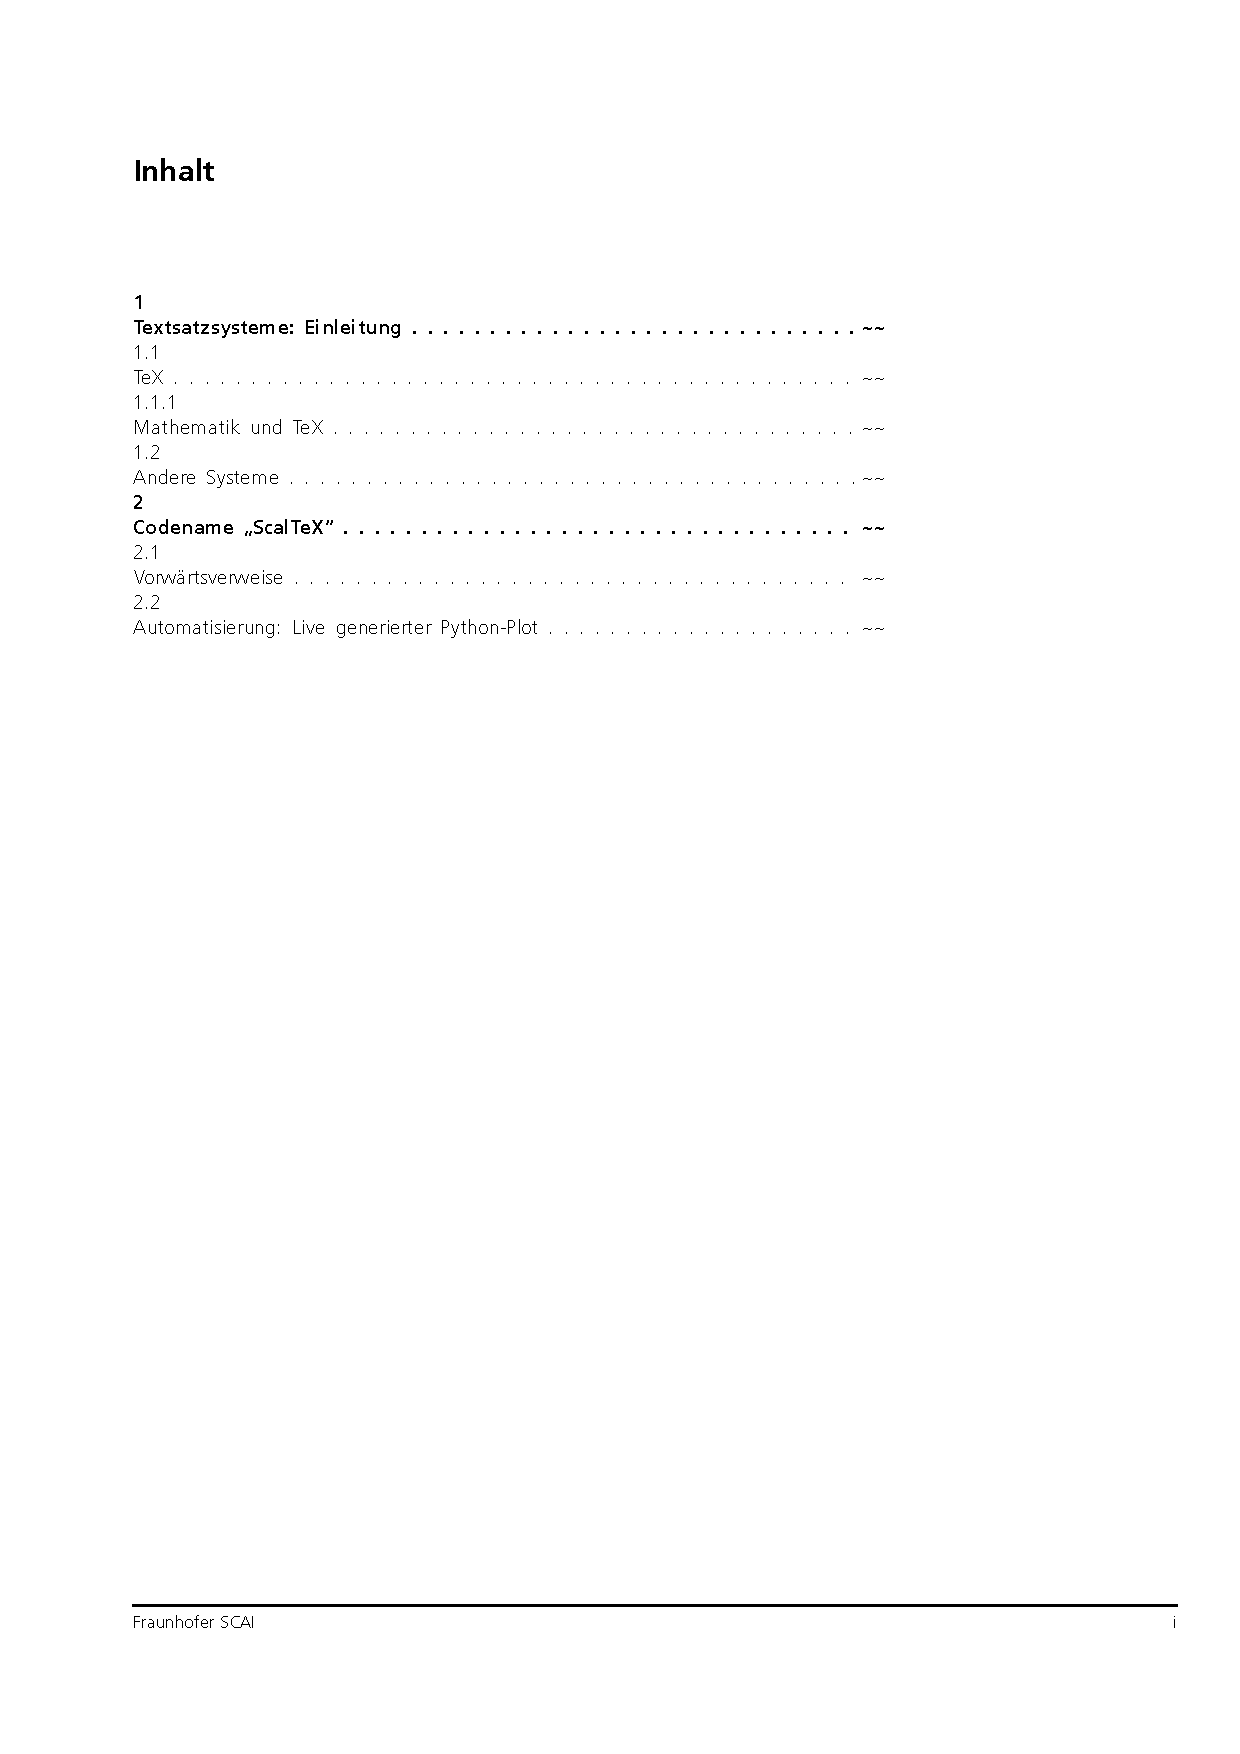
\includegraphics[width=0.9\textwidth]{figures/dsl_skript_0.pdf}
  \caption{Gesetztes Beispiel Inhaltsverzeichnis, Seite i.}\label{fig-dsl_skript_0}
\end{figure}

\begin{figure}[h!]
  \centering
    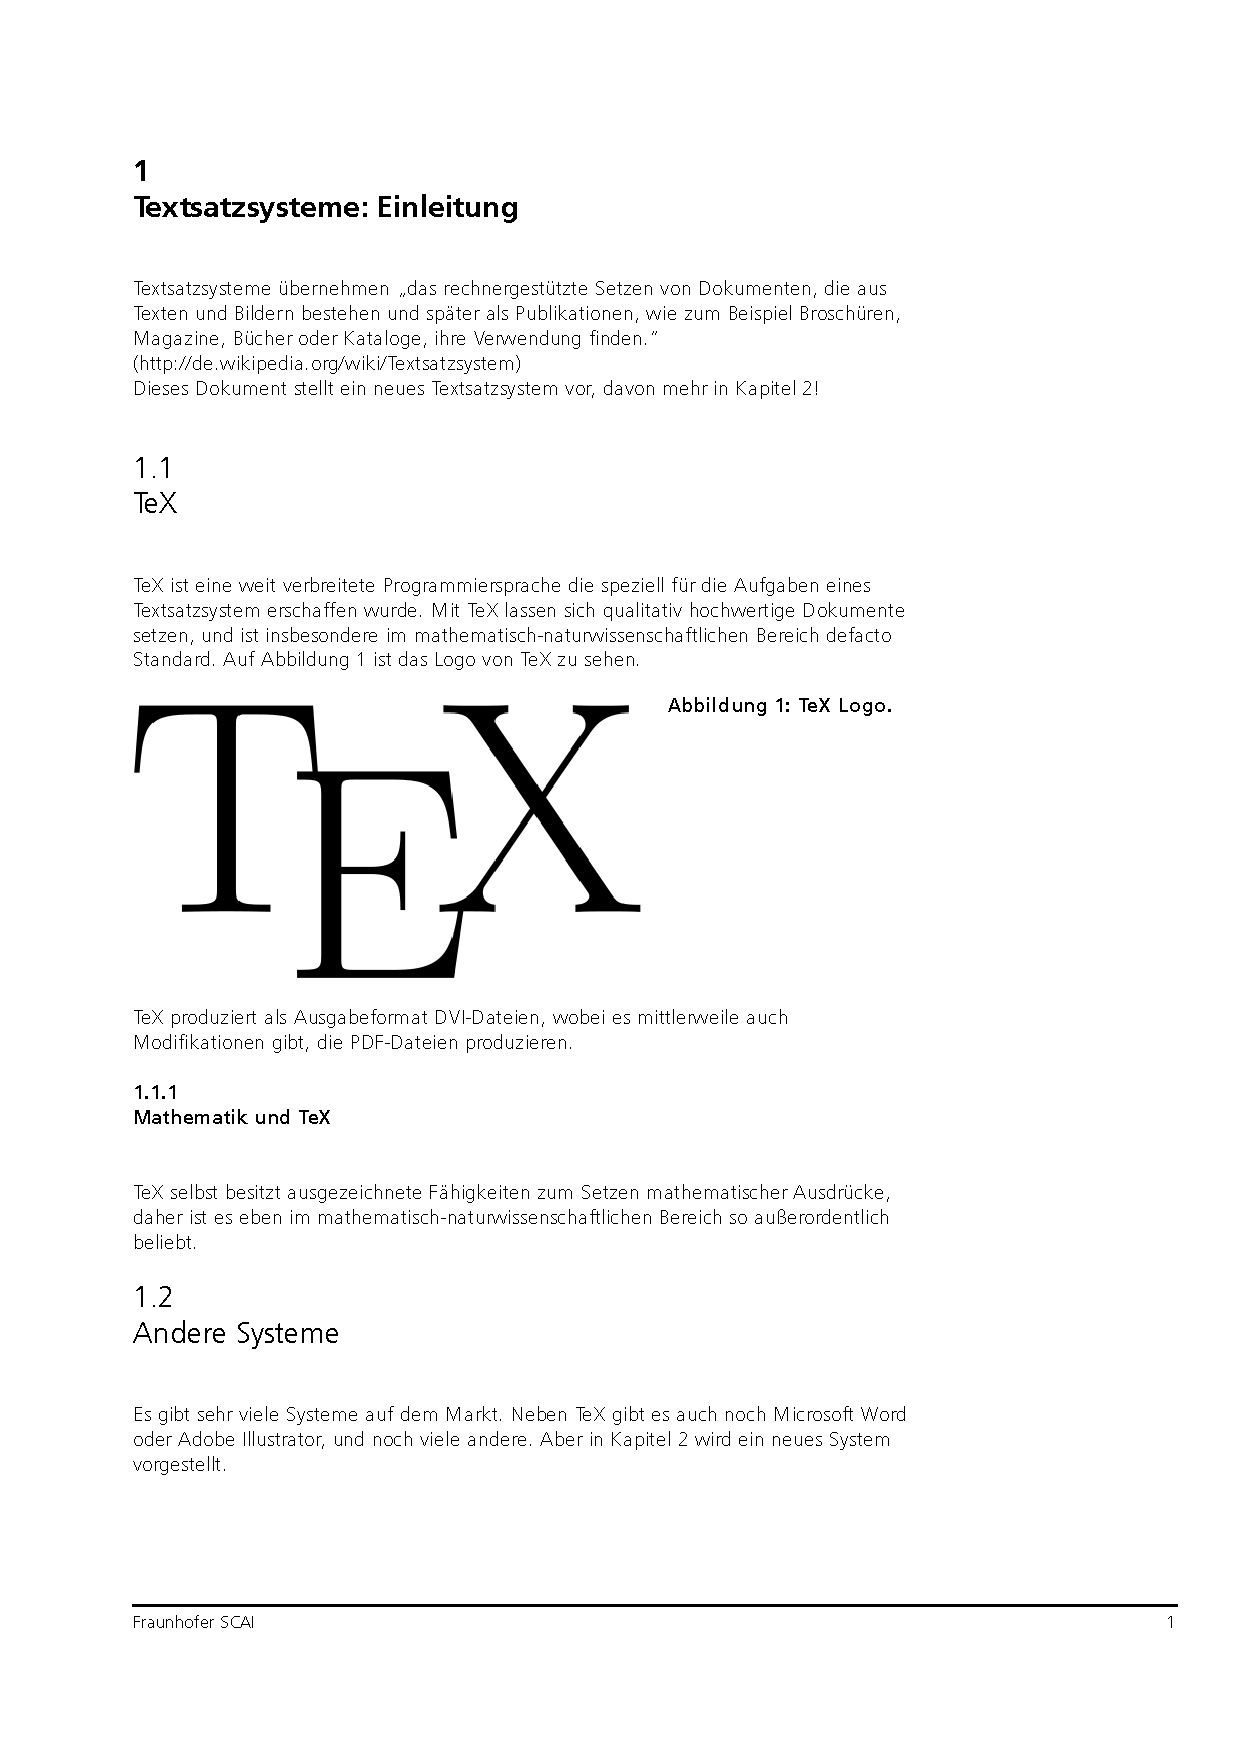
\includegraphics[width=0.9\textwidth]{figures/dsl_skript_1.pdf}
  \caption{Gesetztes Beispiel Kapitel 1, Seite 1.}\label{fig-dsl_skript_1}
\end{figure}

\begin{figure}[h!]
  \centering
    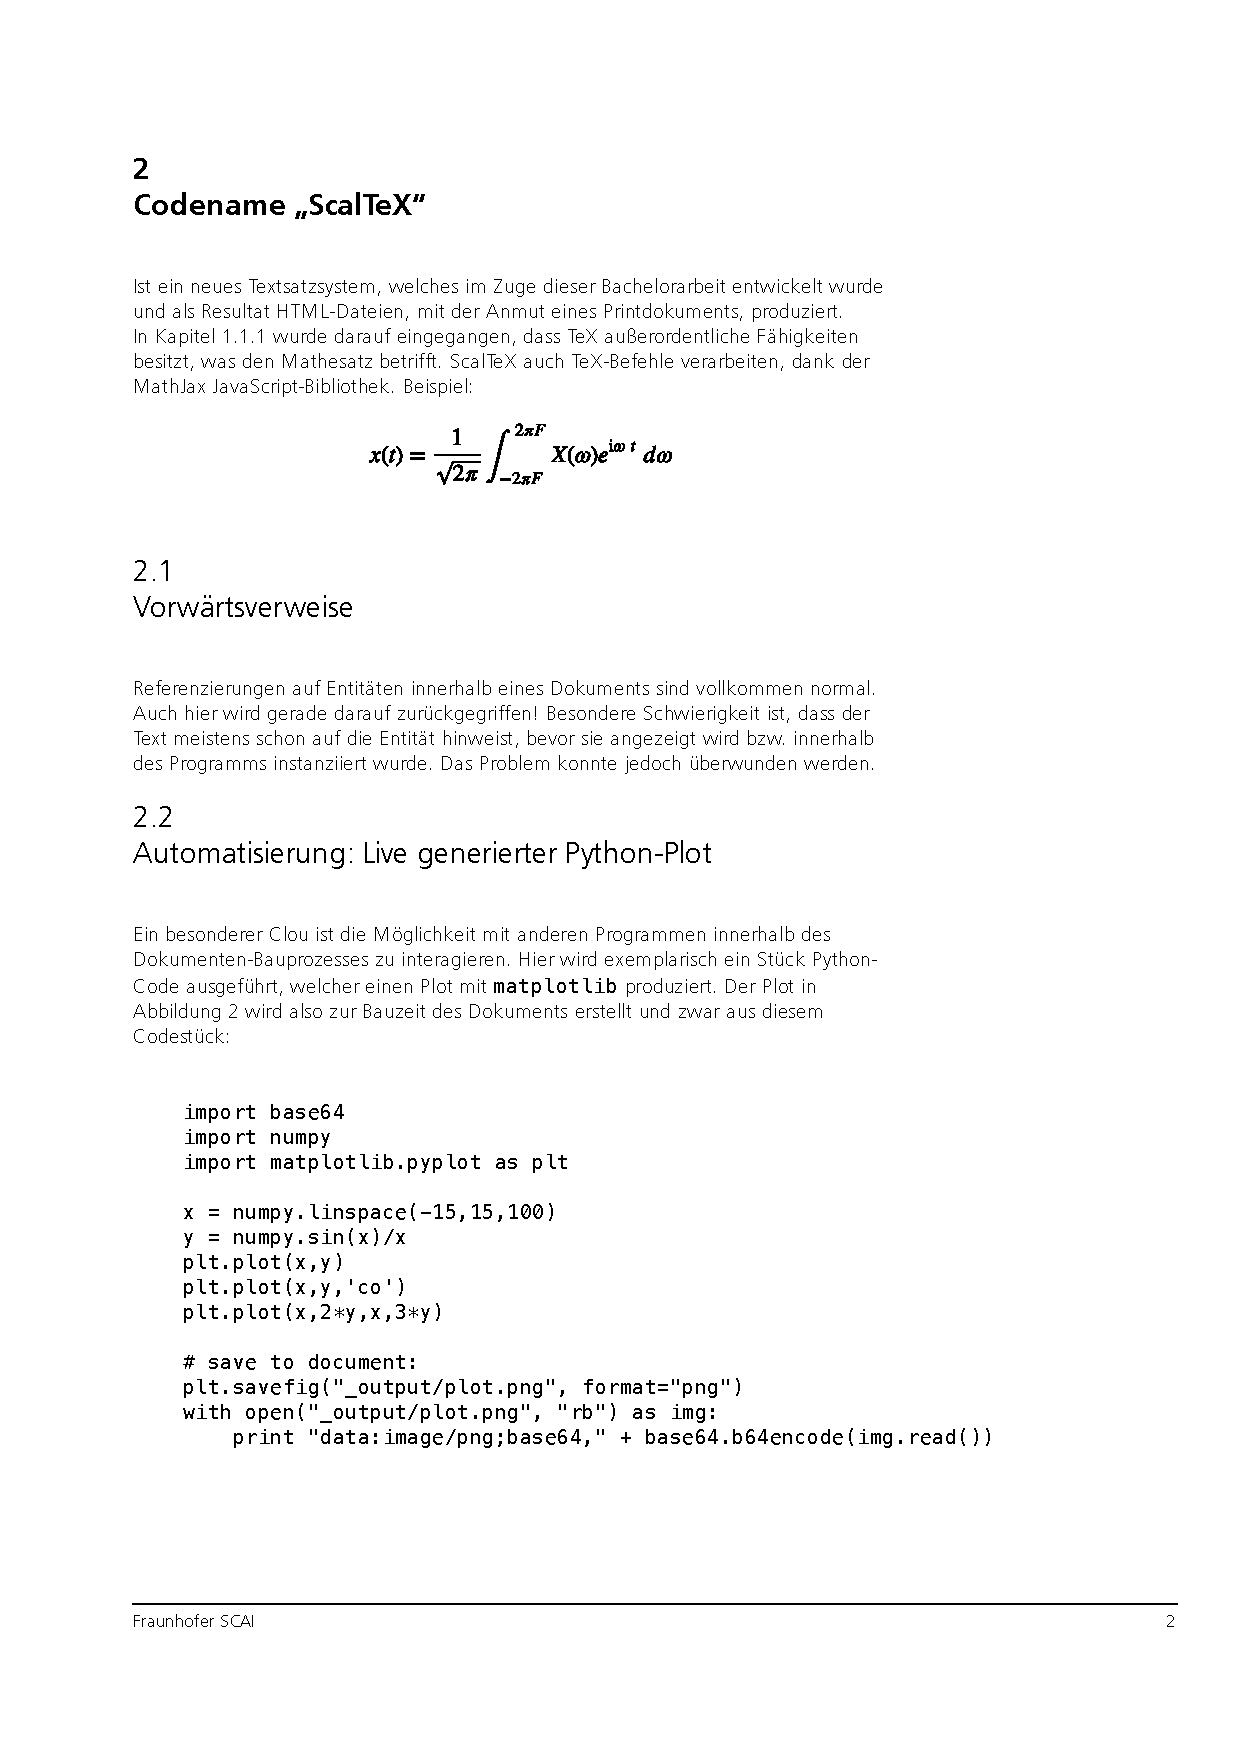
\includegraphics[width=0.9\textwidth]{figures/dsl_skript_2.pdf}
  \caption{Gesetztes Beispiel Kapitel 2, Seite 2.}\label{fig-dsl_skript_2}
\end{figure}

\begin{figure}[h!]
  \centering
    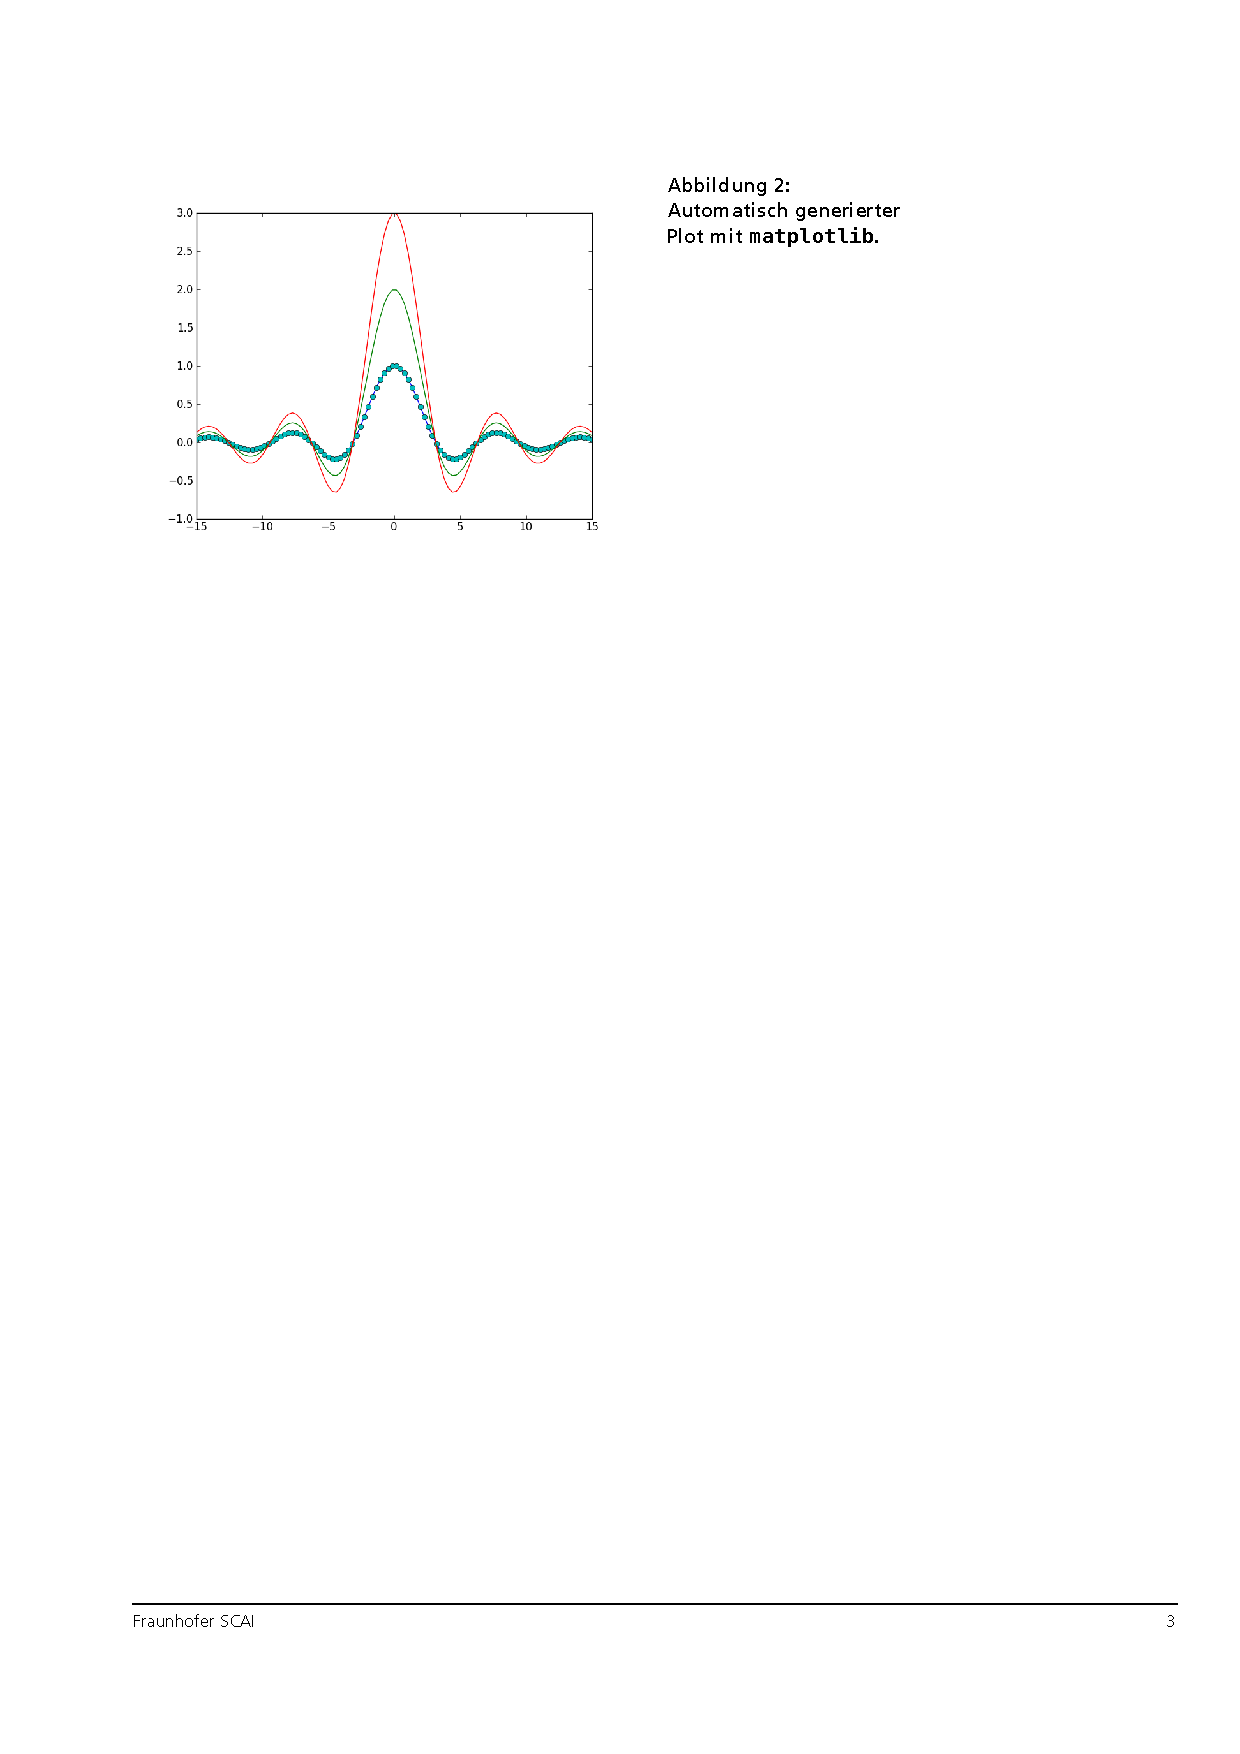
\includegraphics[width=0.9\textwidth]{figures/dsl_skript_3.pdf}
  \caption{Gesetztes Beispiel Kapitel 2, Seite 3.}\label{fig-dsl_skript_3}
\end{figure}
